‘‘\textit{If we knew what we were doing, it would not be called research, would it?}''.

Albert Einstein\\

As Einstein brilliantly put it, research is about travelling in an unknown land, where unknown unknowns mingle with known unknowns, both of which sometimes lie quietly, hidden behind unknown erroneous truths. Think about Ptolemy, admiring his ingenious system that describes how stars and planets orbit around the earth in the not yet called Solar System. Definitely, this held together, like a house of cards; but in a sense, it was a part of the truth, like a flat earth is, in first approximation, true. Indeed, no truth is definitive in Science, which inspired Einstein the following ironical parable:

\textit{``Student:
Dr. Einstein, Aren't these the same questions as last year's final exam?''}

\textit{Dr. Einstein: Yes; But this year the answers are different."}\\

Since a PhD is the first step into the maze of scientific research, this should be anything but a surprise when a PhD does end up far from where it was heading. This is commonly appreciated by considering that what matters (most) is not the end but the initiatory route followed to reach this end. Yet, this adage sounds somewhat vague and should dissatisfy any trained ear, mainly because it does not insist enough on the witty role played by the route itself both on its own edification and on the resulting insights, as argued by \citet{Van-Valen76}, one of the most inspirational evolutionarist ever, in a visionary grant criticism: \textit{`` I have had several useful ideas in biology and mathematics. None were developed under a government grant, and none could have been. I have also had several grants and eventually realised that the required conformity stultified my research}. Wrapped up with contingency and necessity, this evolutionary-like phenomenon holds at any scale of scientific research, from the individual project up to the history of entire fields, not only to its learning stage, and can be likened to Lakatos' concept of research programs fecundity according to which the acknowledgement of a theory relies on its ability to give birth to new research programmes \citep{Lakatos76,Chalmers76}. How much Darwin's ideas were guided by its trip on the Beagle \citep{Darwin45}, its way of collecting facts; and would they have at all emerged had he not boarded on it; no one shall never know. Nor shall we ever know how much they changed the way he did and we do research in Biology, and whether it would have been different had Wallace discovered Evolution alone \citep{Wallace58}.

My PhD work was no exception to this path-dependent pattern, as we shall explain further on, but still, there is more to the story than this universal pattern. To follow its logic requires to go back to its genesis and history, an erstwhile exercise nowadays overlooked in Science, often sacrificed for the sake of both legibility and rationality. At the roots of this project was the idea that cell differentiation, the traditional distinctive trait of multicellular organisms, could have evolved first within unicellular organisms, contrary to the dominant paradigm (see Figure \ref{fig:EvoRoutes-Multi}) according to which complex organisms are cell aggregates that later acquire the ability to differentiate into several cell types. This alternate scenario had already been suggested by \citet{Ispolatov12} and Niklas and Newman \citep{NiklasNewman13,Niklas14}, and is also further supported by the ubiquitous presence of the multicellular genetic toolkit among unicellular organisms \citep{Rokas08,Ruiz-Trillo08,Tikhonenkov20}. What is more, the widespread existence of non-genetic unicellular heterogeneity\footnote{Non-genetic heterogeneity refers to organisms that produce distinctive phenotypes - individuals - from a single genotype. Some authors have been using the term individuality interchangeably with that of heterogeneity \citep{Pradeu16} - even if the first concerns an organism while the latter defines a population - mostly those who do not work on evolutionary questions (\textit{eg.} physiologists, cognitive scientists), what we do not do at this stage for purpose of clarity (we clarify these points in section\textcolor{red}{(à compléter))}.} \citep{Veening08b,Ratcliff10,PaulssonHuh11a,Cerulus16,Takhaveev18} lends further credence to a "differentiation-first" scenario whereby complex multicellular organisms evolved from unicellular ancestors prone to differentiation.

\begin{figure}[h!]
    \centering
    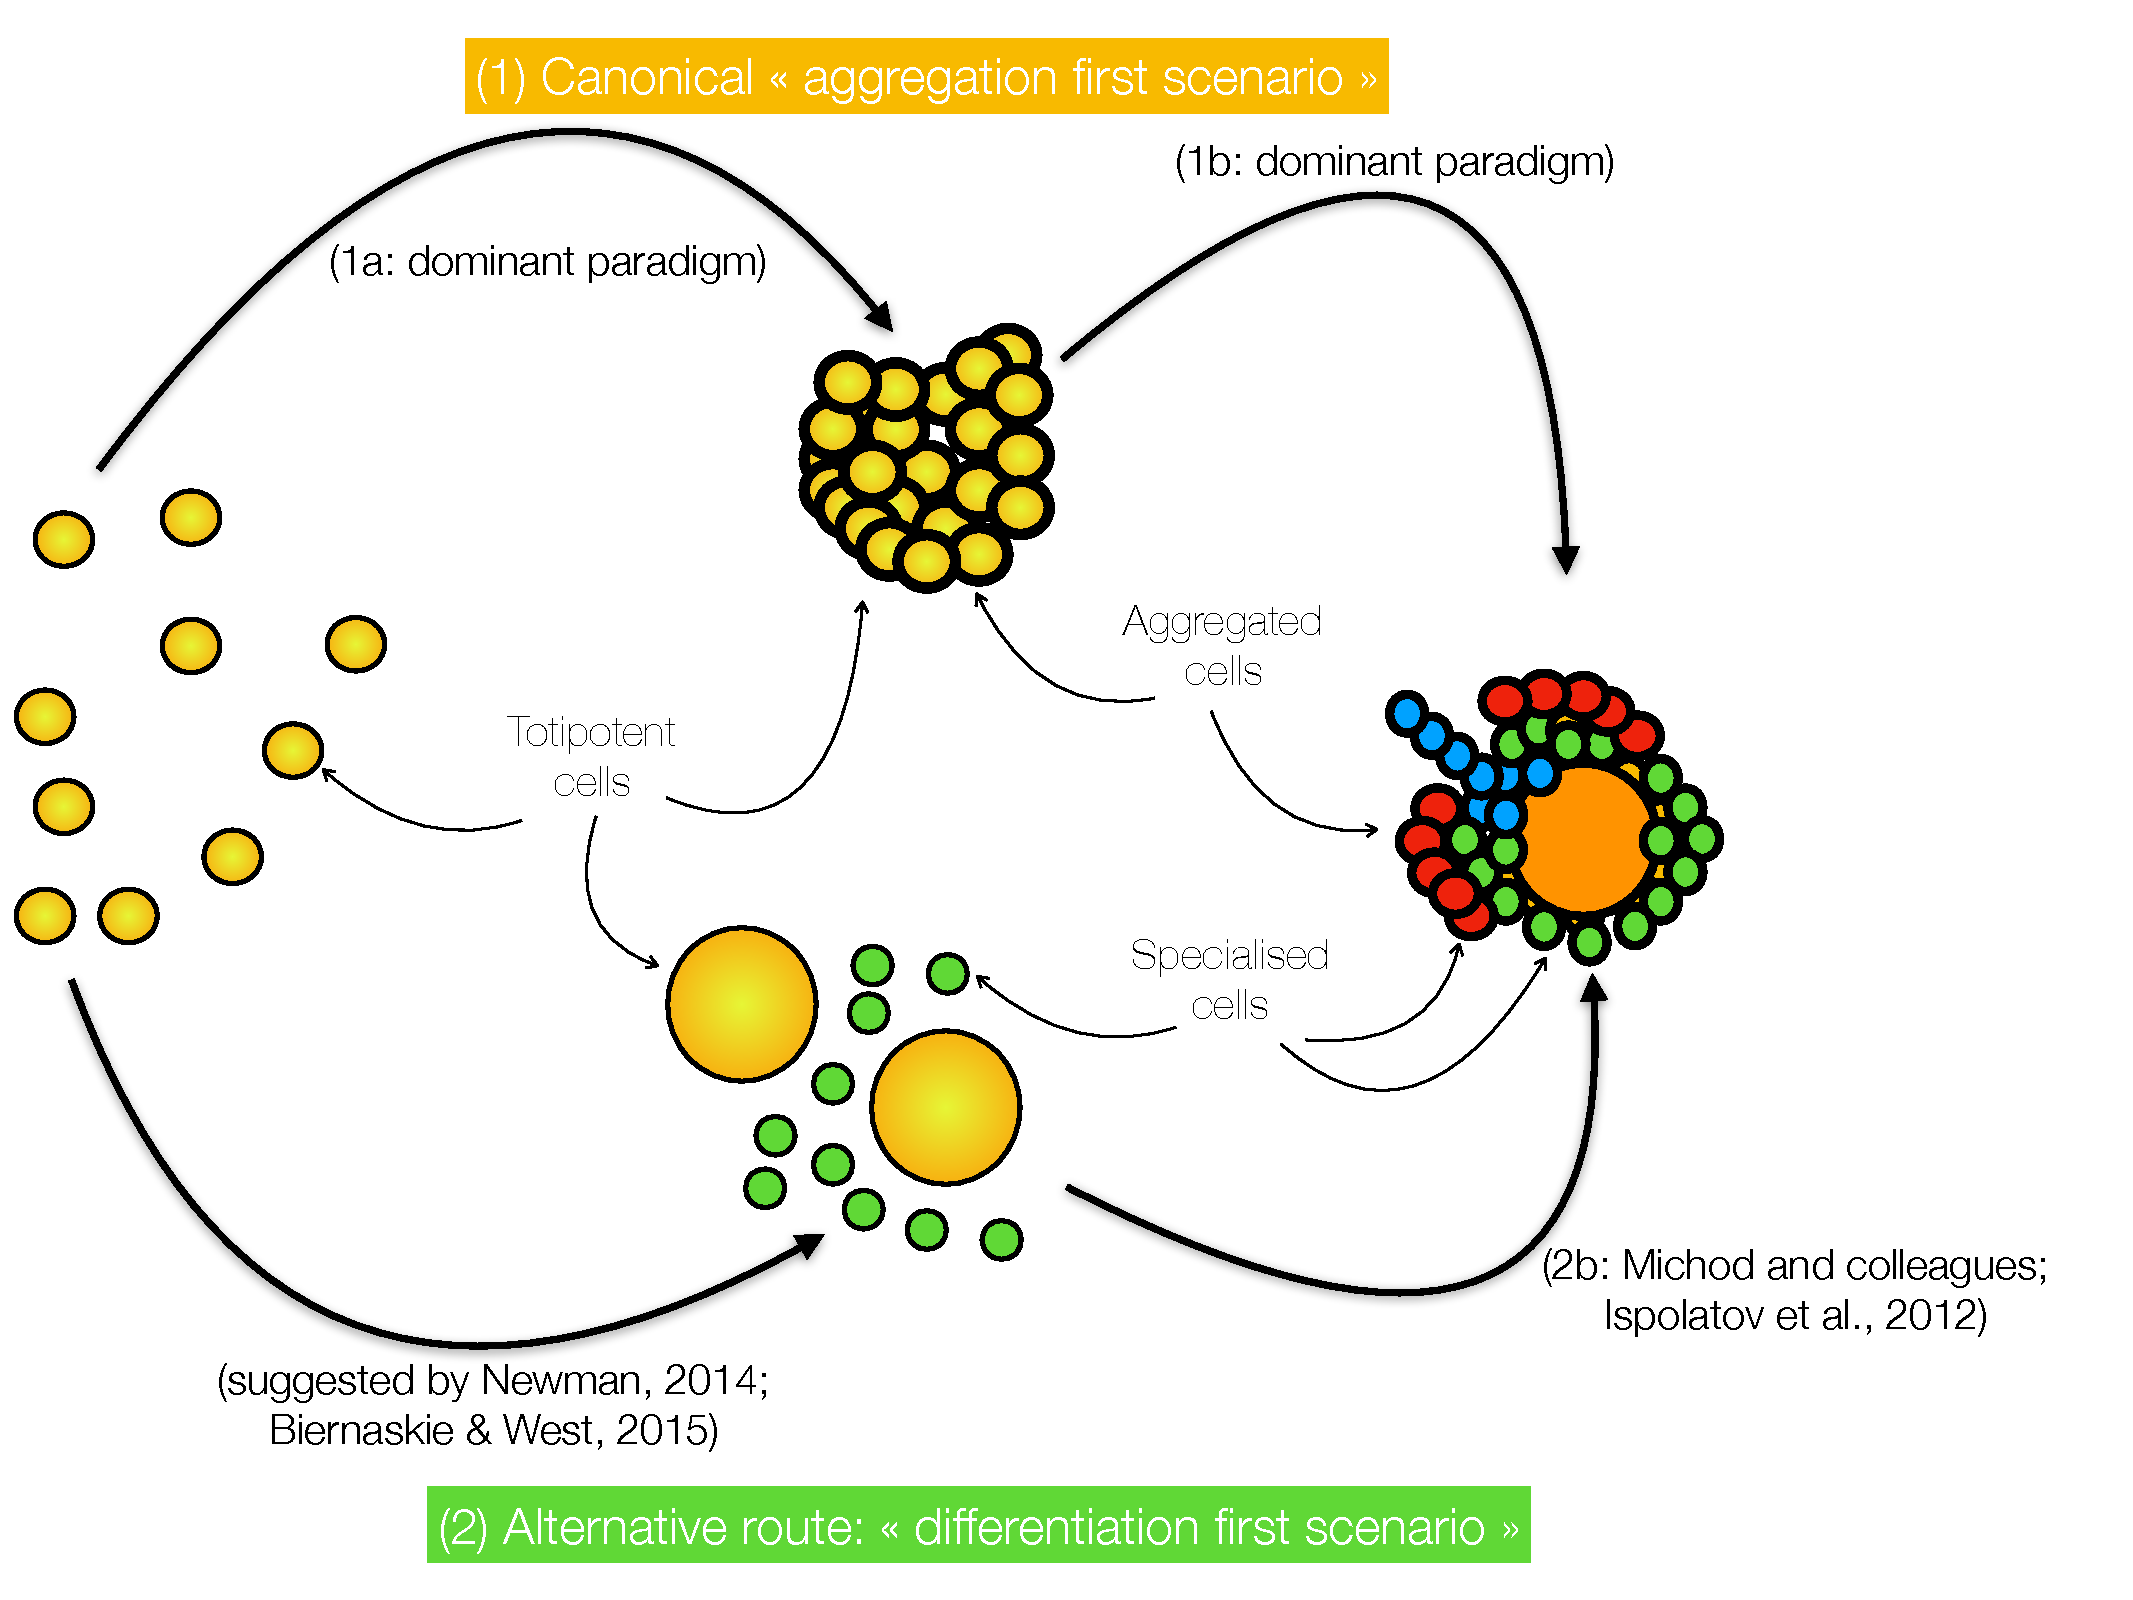
\includegraphics[scale=0.425,trim=0cm 0cm 1cm 0cm,clip]{pics/Cell-Diversity/Schema_route_to_multi.pdf}
    \caption{In the widely accepted "aggregation first scenario", differentiation occurs in already existing aggregates. Recently, \citet{Ispolatov12} have shown that multicellularity could evolve through the cooption of a differentiation behaviour pre-existing in solitary cells. Short after, \citet{BiernaskieWest15} developed a model suggesting coevolution between aggregation and cooperation, triggered by the emergence of aggregation. Meanwhile, \citet{Rokas08}, \citet{Ruiz-Trillo08} and \citet{Tikhonenkov20} have enlightened us about the ubiquitous presence of multicellular toolkit genes among unicellulars \citep{Sebe-Pedros16,Sebe-Pedros17,Ferrer-Bonet17}, and \citet{Niklas14} reminded us that differentiation can be advantageous even for unicellular organisms, which may have therefore paved the way for complex multicellularity \citep{Brunet17}.}
    \label{fig:EvoRoutes-Multi}
    \vspace{-0.5cm}
\end{figure}

For it triggered a dramatic increase in complexity and thereby in diversity, Evolution towards Multicellularity is considered one of the few Major Evolutionary Transitions - METs thereafter - Life came through during its course on earth \citep{Szathmary95,Szathmary15}. More precisely, this is an Evolutionary Transition in Individuality \citep{Michod96,Michod97,West15} - ETI - since it comes with a shift of the level on which Natural Selection operates \citep{Buss87}. During this transition, a transfer of fitness occurs that brings together lower level units into a collective to eventually form a higher level unit \citep{Okasha05,Bourrat15}. We review what makes these transitions special and how they foster Life diversity in section \textcolor{red}{compléter}. Hitherto, insights on ETIs have mostly stemmed from frameworks that rely on arbitrary - and \textit{ad hoc} - fitness functions, aiming to show under which conditions Natural Selection should promote division of labour among lower-level units, and, in turn, drive this transfer of fitness. More specifically, these functions involve two components -- fecundity and survival -- which are supposed to be subject to a trade-off whose convexity determines the benefit conferred by the division of labour \citep{Michod97,Michod05,Rueffler12,Nedelcu12}. Despite being rather artificial, this framework stimulated thoughts and provided the community with qualitative predictions where an explicit trade-off prevails and can readily be captured.

The great philosopher, Bertrand Russell, once said that \textit{the greatest challenge to any thinker is stating the problem in a way that will allow a solution}, and it is very true and even unavoidable. Of course, often in the History of Science, scientists have invented tools to answer their questions. Isaac Newton developed its methods of fluxions\footnote{Fluxion is Newton's equivalent for the (mathematical) differentiation notation concomitantly developed by Leibniz and which went down in history.} to understand the laws of motions \citep{Kleiner01} while Fisher imagined the analysis of variance at the onset of his career when he was starting to study population genetics \citep{Fisher19,Fisher21,Conniffe91}. But no matter how inventive scientists are, the invention still makes them look at their problem through a particular inflexible lens, as it were. In other words, stating the problem in a way that allows a solution impacts not only the solutions we find but also how we interpret these solutions. Thus far, the approach used by scientists interested in ETIs are faced with three closely related limitations. First, it focuses on the effect of an uncharacterized (and unrealistic) preexisting trade-off whereas identifying how it emerges from cellular underpinnings and its ensuing shape remains a conundrum. Meanwhile, how much the chosen definition for fitness - at both levels of individuality - can capture biological reality is anything but clear, to say the least, especially when division of labour facilitates the emergence of and/or exploitation of a new ecological niche. As a corollary, it is hard if not impossible to make quantitative - or even testable - predictions beyond simplistic experiments \citep{Ratcliff12,Bernardes21}. No less importantly, ignoring the mechanisms at the root of the trade-off(s) rules out the possibility for organisms to overcome them through other processes than the transition itself.  Finally, without specifying a genotype-phenotype map - explictly or implicitly - it is impossible to determine the genetic and ecological factors making this transition susceptible to happen (or preventing it). Our original goal was to tackle these issues by adopting a complementary approach based on a mechanistic framework.\\
%Multicellular organisms 

\textit{Yes, fitness is the central concept of evolutionary biology, but it is an elusive concept. Almost everyone who looks at it seriously comes out in a different place.}

Leigh Van Valen\\

Paradoxically, most foundational concepts in Science have proven to be contentious, fleeting and evanescent glimpses teetering as soon as one attempts to get close, akin speed and position which refuse to be captured together at the tiniest scales, questioning their very existence. Sometimes absolute as in Newton's Principia \citep{Greene99,Greene04}, sometimes relative as under Ernst Mach's pen \citep{Greene99,Raine75}, Space and Time have been tossed back and forth ever since They exist, and their ongoing turbulent journey is not finished at all now that they are woven in the same fabric \citep{Einstein05}, for their dimensionality is henceforth standing on the operating table of scientists \citep{Kaluza21,Klein91,Greene04}, awaiting to \textit{explain reality by the impossible} as pointed out by Alexandre Koyré \citep{Koyre73}. No one exactly knows, either, what Money is, other than a belief, nor is the role it plays on economic processes clear: while some proposed that it is purely neutral, especially in the long-run \citep{Friedman95,Hall18,Salerno20}, others thought that burying money to stimulate the creation of industries specialized at unearthing money would be better under certain circumstances such as a job crisis \citep{Keynes36}. Life also had its share of troubles going through the mind of scientists \citep{Schrodinger44,Forterre10,Weber10,,Tessera11}, as more than a hundred propositions have been recorded \citep{Trifonov11}, some of them would now willingly abandon completely the very idea of a definition to rely instead on a fuzzy logic \citep{Bruylants10} more capable to accommodate with a continuous scale from non-life to life and where, following Joseph Felsenstein, \textit{``Rocks [would be] the outgroup''} \citep{Felsenstein03}; but, as coal and oil may not be, one may question : "Which rock is the outgrup, Joe?"

Fitness has definitely earned its place in this distinguished family, and not only because Van Valen is always right. For a long while, Karl Popper denied to Evolution its scientific status on the ground that fitness is a tautology \citep{Popper76}, which it is, as long as one thinks that it is essentially a metrics\footnote{the same argument could be made for time}, as shown by the most basic theorems of Natural Selection \citep{Fisher30,Price72b,Wagner10,Queller17}. Fitness measures the ability of an entity to multiply (not to survive, contrary to a common shortcut) and as such can be the object of a measurement theory \citep{Wagner10} : in a sense, it is the idea that the more one reproduces in a lifetime, the more one will be represented as time goes by, an idea that Popper himself applied to highlight the evolutionary logic behind the scientific approach \citep{Popper72}. If each star -- or cloud, or whatever object one may think to -- gives birth to more stars after it has died, one will see a universe filled with more and more stars: stars would have a high fitness. Recently, the case has incidentally been made that there could be Natural Selection at the level of universes \citep{Smolin97}. At this stage though, it remains effectively untestable. The problem raised by Popper was that fitness measures the ability of an entity to survive but that we determined this ability by measuring the survival, giving rise to a circular reasoning. What makes Evolution a scientific theory is that fitness emerges from mechanistic underpinnings, a case which was recently made by \citet{Doebeli17}, albeit without getting past the metrics problem:  since they only insist on the importance of drawing fitness from birth and death contributions, they do not propose solutions to what fitness is in the first place.

Fitness is the ability of an organism to exploit its environment in order to multiply. Be it to apprehend quantitatively fitness transfers or even the mere effect of Evolution on cell phenotypes, we need to develop an approach where the mapping of phenotypes to fitness genuinely reflects cellular processes and their eventual trade-offs. Cell phenotypes result from the selective expression of proteins through regulatory networks, synchronized production of biomass through intertwined metabolic pathways comprised of enzymes. There have been previous woks where gene network governs the (Hogeweg, Beslon).

In a first work, we built such an evolutionary model where fitness arises from mechanistic underpinnings about genetic, cellular and metabolic processes. This framework is described in the first subsection of results. Using simulations, we demonstrated that  promote the evolution phenotypic heterogenity through , and how this degree of cellular individuality is canalized by the environmental stochasticity. Nevertheless, not knowing the shape of the genotype-phenotype-fitness map keeps from resolving which factors 

It turns out that building such multidimensional metabolic fitness landscapes from a theoretical point of view had not been achieved before. Because some of these dimensions can influence fitness and hence buffer each other weaknesses, they can partly explain why enzyme efficiencies resemble a zoo when gathered together \citep{Bar-Even11}. Along with genetic drift, this dimensionality had long been suggested as a possible explanation for this broad variability \citep{Hartl85,Clark91}. However, we have shown in Subsection \ref{Enzyme-Evolution} (article published in \textit{Molecular Biology and Evolution}) that this explanation is unlikely if not unfounded. Enzyme efficiencies should on the contrary be highly predictable when the mutation-selection-drift has established, while data indicate that they are in fact far more contingent on chemical and metabolic features than related to effective population sizes of organisms. Instead, we have shown that the existence of local metabolic constraints modulate fitness landscapes on which enzymes evolve. These key drivers are extensively studied in Subsection \ref{Enzyme-Evolution}.

Not only are enzyme efficiencies widely distributed, most of them are only moderately efficient and, even more surprisingly, far off their expected physical limits \citep{Bar-Even11,Bar-Even15}. Hence, enzyme efficiencies can be profoundly affected when the cellular content reaches a level that hinders the diffusion of macromolecules (short refs). 

Meanwhile, these moderate enzyme efficiencies significantly depart from the expected population genetics steady-state. As often in biology, this may result from numerous factors, such as the trade-off between protein activity and stability for instance. However, as discussed in the introduction of section (\textcolor{red}{XX}), this latter is unlikely to explain a pattern widely shared among enzymes, as it has been shown to be very enzyme and ecological conditions dependent. Yet, this mutationl load is not entirely unforeseen by theory. In the twilight of the XX$^{eth}$ century, \citet{Hartl96} and \citet{Poon00} have shown that complexity may come at a great cost. 

We discussed 

For quite a while, Science has relied on 
Biology is the science of interactions (citation Smolin)
